% --- Template for thesis / report with tktltiki2 class ---
% 
% last updated 2013/02/15 for tkltiki2 v1.02

\documentclass[finnish]{tktltiki2}

% tktltiki2 automatically loads babel, so you can simply
% give the language parameter (e.g. finnish, swedish, english, british) as
% a parameter for the class: \documentclass[finnish]{tktltiki2}.
% The information on title and abstract is generated automatically depending on
% the language, see below if you need to change any of these manually.
% 
% Class options:
% - grading                 -- Print labels for grading information on the front page.
% - disablelastpagecounter  -- Disables the automatic generation of page number information
%                              in the abstract. See also \numberofpagesinformation{} command below.
%
% The class also respects the following options of article class:
%   10pt, 11pt, 12pt, final, draft, oneside, twoside,
%   openright, openany, onecolumn, twocolumn, leqno, fleqn
%
% The default font size is 11pt. The paper size used is A4, other sizes are not supported.
%
% rubber: module pdftex

% --- General packages ---

\usepackage[utf8]{inputenc}
\usepackage[T1]{fontenc}
\usepackage{lmodern}
\usepackage{microtype}
\usepackage{amsfonts,amsmath,amssymb,amsthm,booktabs,color,enumitem,graphicx}
\usepackage[pdftex,hidelinks]{hyperref}

% Automatically set the PDF metadata fields
\makeatletter
\AtBeginDocument{\hypersetup{pdftitle = {\@title}, pdfauthor = {\@author}}}
\makeatother

% --- Language-related settings ---
%
% these should be modified according to your language

% babelbib for non-english bibliography using bibtex
\usepackage[fixlanguage]{babelbib}
\selectbiblanguage{finnish}

% add bibliography to the table of contents
\usepackage[nottoc]{tocbibind}
% tocbibind renames the bibliography, use the following to change it back
\settocbibname{Lähteet}

% --- Theorem environment definitions ---

\newtheorem{lau}{Lause}
\newtheorem{lem}[lau]{Lemma}
\newtheorem{kor}[lau]{Korollaari}
\theoremstyle{definition}
\newtheorem{maar}[lau]{Määritelmä}
\newtheorem{ong}{Ongelma}
\newtheorem{alg}[lau]{Algoritmi}
\newtheorem{esim}[lau]{Esimerkki}

\theoremstyle{remark}
\newtheorem*{huom}{Huomautus}


% --- tktltiki2 options ---
%
% The following commands define the information used to generate title and
% abstract pages. The following entries should be always specified:

\title{Esimerkkiotsikko}
\author{Eija Esimerkki}
\date{\today}
\level{Seminaariraportti}
\abstract{Tiivistelmä.}

% The following can be used to specify keywords and classification of the paper:

\keywords{avainsana 1, avainsana 2, avainsana 3}
\classification{} % classification according to ACM Computing Classification System (http://www.acm.org/about/class/)
                  % This is probably mostly relevant for computer scientists

% If the automatic page number counting is not working as desired in your case,
% uncomment the following to manually set the number of pages displayed in the abstract page:
%
% \numberofpagesinformation{16 sivua + 10 sivua liitteissä}
%
% If you are not a computer scientist, you will want to uncomment the following by hand and specify
% your department, faculty and subject by hand:
%
% \faculty{Matemaattis-luonnontieteellinen}
% \department{Tietojenkäsittelytieteen laitos}
% \subject{Tietojenkäsittelytiede}
%
% If you are not from the University of Helsinki, then you will most likely want to set these also:
%
% \university{Helsingin Yliopisto}
% \universitylong{HELSINGIN YLIOPISTO --- HELSINGFORS UNIVERSITET --- UNIVERSITY OF HELSINKI} % displayed on the top of the abstract page
% \city{Helsinki}
%


\begin{document}

% --- Front matter ---

\maketitle        % title page
\makeabstract     % abstract page

\tableofcontents  % table of contents
\newpage          % clear page after the table of contents


% --- Main matter ---

\section{Johdanto}
\section{Web-ontologiakieli OWL}

pieni alustus, että miksi käsitellään owl ja mitä konstruktioita tarvitsemme owl-s:n ymmärtämiseen

\subsection{Teknologiat, jotka mahdollistavat OWL:n}
\subsubsection{XML}

onko tarpeen?

\subsubsection{RDF/RDFS}

\subsection{tarpeelliset OWL-konstruktiot OWL-S:n ymmärtämiseen}

luokka

instanssi

suhde

import


\section{Webpalveluiden kuvauskieli OWL-S}

UDDI

\subsection{Korkean abstraktiotason rakenne}

Palveluontologian korkean abstraktiotason rakenne muodostuu kolmen tyyppisestä tiedosta ja ne vastaavat kolmeen eri kysymykseen \cite{OWLS}:

\begin{itemize}

  \item \textit{Mitä palvelu tarjoaa mahdolliselle asiakkaalle?} Tähän antaa vastauksen ontologian \textit{profiili}, joka kertoo karkealla tasolla mitä palvelu tarjoaa. Profiilin 
 avulla palveluntarjoaja voi mainostaa palveluaan potentiaalisille asiakkaille. Profiilissa kerrotan myös, \textit{kuka} palvelun tarjoaa. Jokainen \texttt{Service}-luokka edustaa yhtä \texttt{ServiceProfilea} \cite{OWLS}.
 
 \item \textit{Kuinka palvelua käytetään?} Ontologian \textit{prosessimalli} antaa vastauksen tähän ja se esitetään luokassa \texttt{ServiceModel}. Palvelun ja sen prosessimallin 
 välillä on \texttt{describedBy} -suhde\cite{OWLS}. 
 
 \item \textit{Miten palvelun kanssa kommunikoidaan?} Tähän antaa vastauksen ontologian \textit{maadoitus}, jossa määritellään esimerkiksi tuki erilaisille viestiprotokollille. 
 \texttt{Service} -luokalla on ominaisuus \texttt{supports}, joka viittaa \texttt{ServiceGrounding} -luokkaan\cite{OWLS}.  
 
 \begin{figure}[ht]
 \centering
 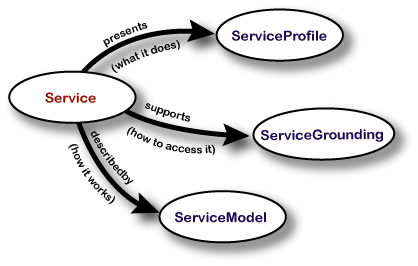
\includegraphics[scale=0.60]{karkea_taso.png}
 \caption{OWL-S:llä kuvatun palveluontologian korkean taon rakenne \cite{OWLS}}
 \label{karkea_taso}
\end{figure}
 
 Kuten kuvasta \ref{karkea_taso}  voidaan nähdä, jokaista julkistettua palvelua kohden on yksi \texttt{Service}-luokan instanssi, joka edustaa \texttt{ServiceProfilea} suhteella \texttt{presents}, on \texttt{ServiceModel}in kuvailema suhteella \texttt{describedBy} ja \texttt{serviceGrounding}in tukema suhteella \texttt{supports}.
 
\end{itemize}


\subsection{Profiili}

Profiili siis kertoo mitä palvelu tekee ja kuka palvelun tarjoaa. Se mahdollistaa asiakkaita (agentteja) löytämään palvelun esimerkikisi keskitetyistä palvelurekistereistä kuten UDDI tai puhtaan P2P:n puitteissa. 
Profiili tarjoaa kolmenlaista informaatiota \cite{OWLS}:

\begin{enumerate}
 \item \textit{Tuottajainformaatio} kertoo tietoja palvelun tuottajasta, esimerkiksi ylläpitäjän tai asiakasyhteyshenkilön yhteystiedot. Myös lyhyt tekstikuvaus palvelusta sekä yksikäsitteinen nimi palvelulle määritellään profiilissa\cite{OWLS} .
 
 \item \textit{Toiminnallinen kuvaus} kuvaa (tautologia) palvelun käyttämät \textit{syötteet}, sen tuottamat \textit{tulosteet}, \textit{esiehdot}, jotka tulee olla voimassa ennen määrättyjä
 prosesseja sekä \textit{tilamuutoksia}, joita prosessien suorittaminen aiheuttaa \cite{OWLS}. ESIMERKKEJÄ?? Nämä samat käsitellään myös prosessimallissa, mutta tarkemmalla tasolla. OWL-S ei aseta
 rajoitteita sen suhteen, onko profiili ja prosessimalli konsistentit toisiinsa nähden, mutta ollakseen totuudenmukainen palvelun tarjoamien todellisten palvelujen suhteen, tulee profiilin ilmaista
 palvelut yhtenevästi prosessimallin suhteen. 
 
 \item \textit{Toimintaa kuvaavat ominaisuudet} ?? Ensinnäkin palvelu voidaan luokitella jonkun tunnetun luokittelun, esimerkiksi UNSPSC:n [footnote] mukaan. Toiseksi, palvelun laatuluokitus voidaan 
 ilmaista profiilissa. Profiilin lopussa on määrittelemätön määrä parametreja, joilla voidaan kertoa esimerkiksi palvelun maantieteellisestä saatavuudesta, arvioidusta vasteajasta jne. \cite{OWLS}.
\end{enumerate}

Seuraavassa käsitellään em. kolmea osa-aluetta sekä profiilitiedoston rakenne tarkemmin. 

\subsubsection{Ontologioiden tuonti ja viitteet prosessimalliin sekä palveluun}

Profiilin(-tiedoston) alussa voidaan tuoda ontologian käyttöön muita jo määriteltyjä ontologioita tavallisilla owl:n \texttt{imports}-lauseilla. Esimerkissä tuodaan palvelun pääasiallinen määritelmä \texttt{BravoAirService} ontologian käyttöön\cite{daml}:  

\begin{verbatim}
<owl:imports rdf:resource="http://www.daml.org/services/owl-s/1.2/BravoAirService.owl"/>
\end{verbatim} 

Jokaista profiilia edustaa palvelu. Viittaus palvelun määritelmään ilmaistaan \texttt{presentedBy}-suhteella\cite{daml}: 

\begin{verbatim}
<service:presentedBy rdf:resource="http://www.daml.org/services/owl-s/1.2/BravoAirService.owl#BravoAir_ReservationAgent"/> 
\end{verbatim} 

\subsubsection{Tuottajainformaatio}

Palveluntarjoajan yhteystiedot on tarkoitettu pääasiassa ihmisten luettavaksi. Yhteyshenkilöitä voidaan luonnollisestikin määritellä useita, esimerkissä ainoastaan yksi\cite{daml}:  

\begin{verbatim}
<profile:contactInformation>
  <actor:Actor rdf:ID="BravoAir-reservation">
  <actor:name>BravoAir Reservation department</actor:name>
  <actor:title>Reservation Representative</actor:title>
  <actor:phone>412 268 8780</actor:phone>
      . . .
  </actor:Actor>
</profile:contactInformation>
\end{verbatim} 

Yteystietoihin kirjataan usein ylläpitäjän ja/tai kaupallisen edustajan tietoja. 

Palvelun tekstikuvaus kirjoitetaan \texttt{textDescription}-tägin ja nimi \texttt{serviceName}-tägin sisään.  


\subsubsection{Toiminnallinen kuvaus}

Toiminnallinen kuvaus ilmaisee mitä toimintoja palvelu tarjoaa ja minkä ehtojen puitteissa. OWL-S \texttt{Profile} ilmaisee kahdenlaista funktionaalisuutta: syötteet ja tulosteet, jotka voidaan ajatella informaatiovirtoina sekä esiehdot ja vaikutukset, jotka voidaan ajatella tilamuutoksina. Edellisiä vastaavat owl-ominaisuudet ovat\cite{OWLS}:

\textbf{hasInput}, joka saa arvokseen \texttt{Process}-ontologiassa määriteltyjä \texttt{Input}-luokan ilmentymiä. 


\textbf{hasOutput}, joka saa arvokseen \texttt{Process}-ontologiassa määriteltyjä \texttt{Output}-luokan ilmentymiä


\textbf{hasPrecondition}, joka määrittelee jonkin esiehdon, joka on luokan \texttt{Precondition} ilmentymä


\textbf{hasresult}, joka ilmaisee minkä ehtojen puitteissa tuloksia generoidaan sekä ja mitä tilamuutoksia prosessien suoritus saa aikaan. Saa arvokseen \texttt{Result}-luokan ilmentymiä.  

Alla olevassa esimerkissä on määritetty, että prosessilla on syöte ''lähtökenttä'' (\textit{departureAirport}), tuloste ''lentoja löytynyt'' (\textit{FlightsFound}) ja 
tilamuutos ''istumapaikka löytynyt'' (\textit{HaveSeatResult})\cite{daml}:

\begin{verbatim}
 <profile:hasInput rdf:resource="http://www.daml.org/services/owl-s/1.2/BravoAirProcess.owl#DepartureAirport"/
 <profile:hasOutput rdf:resource="http://www.daml.org/services/owl-s/1.2/BravoAirProcess.owl#FlightsFound"/>
 <profile:hasResult rdf:resource="http://www.daml.org/services/owl-s/1.2/BravoAirProcess.owl#HaveSeatResult"/
\end{verbatim}

Edellisessä esimerkissä on poimittu ainoastaan muutamia toiminnallisia määrityksiä, todelliset määritykset voi katsoa liitteestä nnn. 

\subsubsection{Toimintaa kuvaavat ominaisuudet}




\subsection{Prosessi}

\subsection{Maadoitus}
% Write some science here.

Esimerkkilause ja lähdeviite~\cite{pitfalls}.


% --- Back matter ---
%
% bibtex is used to generate the bibliography. The babplain style
% will generate numeric references (e.g. [1]) appropriate for theoretical
% computer science. If you need alphanumeric references (e.g [Tur90]), use
%
% \bibliographystyle{babalpha-lf}
%
% instead.

\bibliographystyle{babplain-lf}
\bibliography{references-fi}


\end{document}
